\documentclass[11pt]{article}
\usepackage[top=2.5cm,bottom=2.5cm,right=2.5cm, a4paper]{geometry}                % See geometry.pdf to learn the layout options. There are lots.
%\geometry{a4paper}                   % ... or a4paper or a5paper or ... 
%\geometry{landscape}                % Activate for for rotated page geometry
%\usepackage[parfill]{parskip}    % Activate to begin paragraphs with an empty line rather than an indent
\usepackage{amssymb}
\usepackage{authblk}
	\renewcommand\Authands{ \& }
\usepackage{graphicx}
\usepackage{epstopdf}
\usepackage[hidelinks]{hyperref}
\usepackage[utf8]{inputenc}
\usepackage[ttscale=.875]{libertine}
\usepackage{multicol}
\usepackage{natbib}
\DeclareGraphicsRule{.tif}{png}{.png}{`convert #1 `dirname #1`/`basename #1 .tif`.png}

\title{Spatial autocorrelation in biogeography: a methodological update}
%\title{Averaging statistical models: How does it work and when should we use it?}
\author[1]{Carsten F. Dormann\thanks{corresponding author; Tennenbacher Str. 4, 79106 Freiburg, Email: \url{carsten.dormann@biom.uni-freiburg.de}}}
\author[1]{Severin Hauenstein}
\affil[1]{Biometry and Environmental System Analysis, University of Freiburg, Germany}

\date{\today}                                           % Activate to display a given date or no date

% Colin Beale: R-INLA, 
% Petr Keil: trend-surface-GAM instead of SEVM

\begin{document}
\maketitle
\frenchspacing

\tableofcontents

\begin{abstract}

\end{abstract}

\section{Introduction}
Biogeographical data often display spatial patterns. This is largely due to \emph{spatial dependence}, i.e. the fact that the environment changes smoothly, and the distribution of species is dependent on this spatially autocorrelated environment. A statistical model accounting for these environmental predictors will thus have residuals that are not spatially autocorrelated any more. However, there are two other common sources of spatial patterns: biological processes (such as dispersal, territoriality) and model misspecification (such as omitting an important predictor or representing a non-linear relationship by a linear term). The key diagnostic feature for a pathological model is thus spatial autocorrelation of model residuals.

Once such residual spatial autocorrelation (rSA) is detected, different statistical methods are available to embrace the pattern and represent it as part of the statistical model.\footnote{We carefully avoid the term `nuisance' here, because we actually may learn something from rSA and see it as part of the information, not as distracting noise. Still, from a purely statistical point of view, we have to meet the model assumptions of i.i.d. and hence need to represent it in the model.} Ten years ago, \citet{Dormann2007} published a review of the methods available at that time to deal with spatial autocorrelation. Since then, the range of possible techniques has increased dramatically, and present now a more bewildering diversity than ever before. 

The aim of this publication is to pull together methods available in open-source software, demonstrate how to apply them to a common data set, and help the interested user decide which to choose. We do not attempt to present a comparison of the quality of these methods, because that depends on the questions asked, the data available, the computing infrastructure, but a set of criteria to consider. In fact, we strongly recommend using multiple methods whenever logistically possible, if only because we sometimes do not have enough experience with them to fully understand their strengths and weaknesses.

\section{What spatial modelling approaches exist?}

Classes of approaches:
\begin{enumerate}
\item modelling the variance-covariance matrix, with the maximal underlying general model structure $y \sim \rho W y + X \beta + \lambda W u + \varepsilon$. This equation contains an autoregressive term, i.e. a part of the right-hand side that is a function of the response ($\rho W y$), the ordinary regression predictors ($X\beta$) and a spatial autocorrelation term in the error ($\lambda W u$). $\varepsilon$ is the i.i.d. error, while $u$ is the autocorrelated error term. Approaches now differ in which terms are actually modelled, and how the weights matrix $W$ is parameterised.%(GLS, CAR/SAR, autocovariate, INLA, spBayes, CAR.proper (BUGS), GEE)
In particular, the weights matrix $W$ can be parameterised \emph{marginally}, i.e. alongside the model parameters, yielding the class of simultaneous autoregressive models, or \emph{conditionally}, i.e. conditional on the model parameters, yielding the class of conditional autoregressive models (see references in Hogan \& Tchernis 2004, p. 317 left).
\begin{enumerate}
	\item Simulataneous autoregressive model (SAR) is a special case, where the spatial autocorrelation in $y$ can be attributed entirely to the model's error term: $y \sim X\beta + \lambda W u + \epsilon$ (\texttt{spdep::errorsarlm}, \texttt{McSpatial::sarml}).
	\item SAR models with a lag, i.e. $y \sim X\beta + \lambda W u + \varepsilon$ (spdep::lagsarlm) or full ``mixed'' model with both sources of spatial errors: $y \sim \rho W y + X\beta + \lambda W u + \epsilon$ (\texttt{sphet}, \texttt{spdep::errorsarlm(., etype="mixed")})
	\item Conditional autoregressive model (CAR) represents the case, where $y \sim X\beta + \rho W (Y - X\beta) + u, u \sim N(0, \Sigma)$; it is similar to the lagged SAR but uses the residuals for the lag, and it still has a potentially autocorrelated error $u$ represented by variance-covariance matrix $\Sigma$ (\texttt{spdep::spautolm}, \texttt{CARBayes} [binomial \& Poisson], \texttt{hSDM::hSDM.binomial.iCAR} [binomial])
	\item autologistic (or more generally: autocovariate) regression, is the case where the term $Wy$ is computed before fitting the model and then added as another predictor to $X$, and it is thus also a conditional autoregressive model (\texttt{ngspatial::autologistic}; as JAGS model with multivariate normal latent response [any distribution]; \texttt{spdep::autocov\_dist}; \texttt{spatcounts::est.sc} [(generalised) Poisson, neg. binom., ZIP, ZIGP]); 
	\item Generalised Least Squares, with the underlying model $y \sim X\beta + \Sigma$, where $\Sigma$ is the variance-covariance matrix, which is modelled as a function of spatial configuration (e.g. exponentially decreasing with distance D: $\Sigma \sim e^{-\delta D}$) (\texttt{nlme::gls} [Gaussian], \texttt{ramps::georamps} [Gaussian]).
	\item Generalised Estimation Equations (GEE) can be used to parameterise the variance-covariance matrix $\Sigma$, either flexibly or more in a fixed structure (\texttt{gee}, \texttt{geepack::geese}).
\end{enumerate} 
\item invent missing variables: SEVM/PCNM, wavelet, latent variable stuff from Guillaume (Canadian Ovaskainen-postdoc); more recently, \citet{Crase2013} proposed to use the residuals of a model to compute the autocovariate, as the CAR does, too; %(which is conceptually similar to a regularisation of the autocovariate, as then only the part unexplained by the predictors is modelled as autocovariate);
\item address spatial autocorrelation as non-stationarity problem, using spatially variable coefficient models, or geographically weighted regression (\texttt{GWmodel::gwr.basic}, \texttt{gwrr::gwr.est}, \texttt{spgwr::gwr}, \texttt{McSpatial::cparlwr}, \texttt{mgcv::gam(...  s(x, y, by=x1))};
\item for point (presence-only) data: iPPM with interaction; LGCP
\item trend-surface regression; this typically only represent coarse-scale, longer-range spatial structures, and generally will bias model parameters if implemented only as spatial polynomials (it requires a regularisation approach, as implemented e.g. in GAMs).
\item others: Mátern correlation model (\texttt{spaMM::corrHLfit})
\end{enumerate}

\begin{table}
\caption{Overview of spatial regression approaches.} \label{tab:approaches}
\hspace{-1cm}
\begin{tabular}{lp{8cm}p{4cm}}\hline
Method  &  software & references \\\hline
autocovariate regression  & spdep; ngspatial::autologistic; dynamic autologistic using JAGS: Guelat-code (footnote)  & Besag, Bardos\\ % David Bardos
CAR & CARBayes; hglm; hSDM; PReMiuM; spdep; spatcounts; sphet &\\			% Jerome Guelat?
GEE & gee; geepack::geese & \\ 						 			% Gudrun Carl
GLS/GLMM/GAMM & ngspatial::sparse.sglmm; nlme; regress; spaMM; spBayes; spatcounts & Finley \\ % Andy Finley
GWR & GWmodel; gwrr; McSpatial; spgwr; GWLelast &\\  			% Roger Bivand?
INLA & R-INLA &\\ 									 			% Colin Beale, Maria-Grazia Pennino
latent predictor & HMSC & Blanchet\\ 				 			% Guillaume Blanchet
SAR (error, lag, mixed) & hglm; spdep::GMerrorsar, spdep::errorsarlm; sphet? &\\ % ?
SEVM/PCNM & vegan::pcnm; AEM; PCNM; spdep::ME & \\ % Pedro Peres-Neto
RAC (residual autocovariate) & & \citet{Crase2013}\\ 			% Beth Crase/Brendan Wintle
spatial wavelets  & biwavelet; brainwaver; rwt; wavelets; waveslim; wavethresh & \citet{Carl2007,Carl2008}\\ % Gudrun Carl
spatial BRT & & Hothorn et al. 2011 \\ 							% Torsten Horthorn? Boris Schröder?
?geostatistical models? & geoRglm; ramps; spacom; spatialkernel &\\ % Justin Calabrese?
?spatial factor analysis? & SpatialFA & Thorson et al. 2015 MEE\\   % ?
trend-surface regression & GLM; mgcv::gam & \\\hline 			% Petr Keil, Simon Wood
non-spatial references & GLM, randomForest, ANN &\\
\hline
\end{tabular}
(\url{http://rstudio-pubs-static.s3.amazonaws.com/9687_cc323b60e5d542449563ff1142163f05.html})
\end{table}


\section{Methods}

\subsection{Simulating spatial autocorrelation}
We created data sets along three experimental dimensions: (I) kind of landscape; (II) cause of SA; and (III) type of distribution of the response variable.

Landscapes were either smooth, realistic-random or real, to evaluate whether simple configurations of $X$ yield similar results as real landscapes. (Fig.~\ref{fig:landscapes}).

\begin{figure}
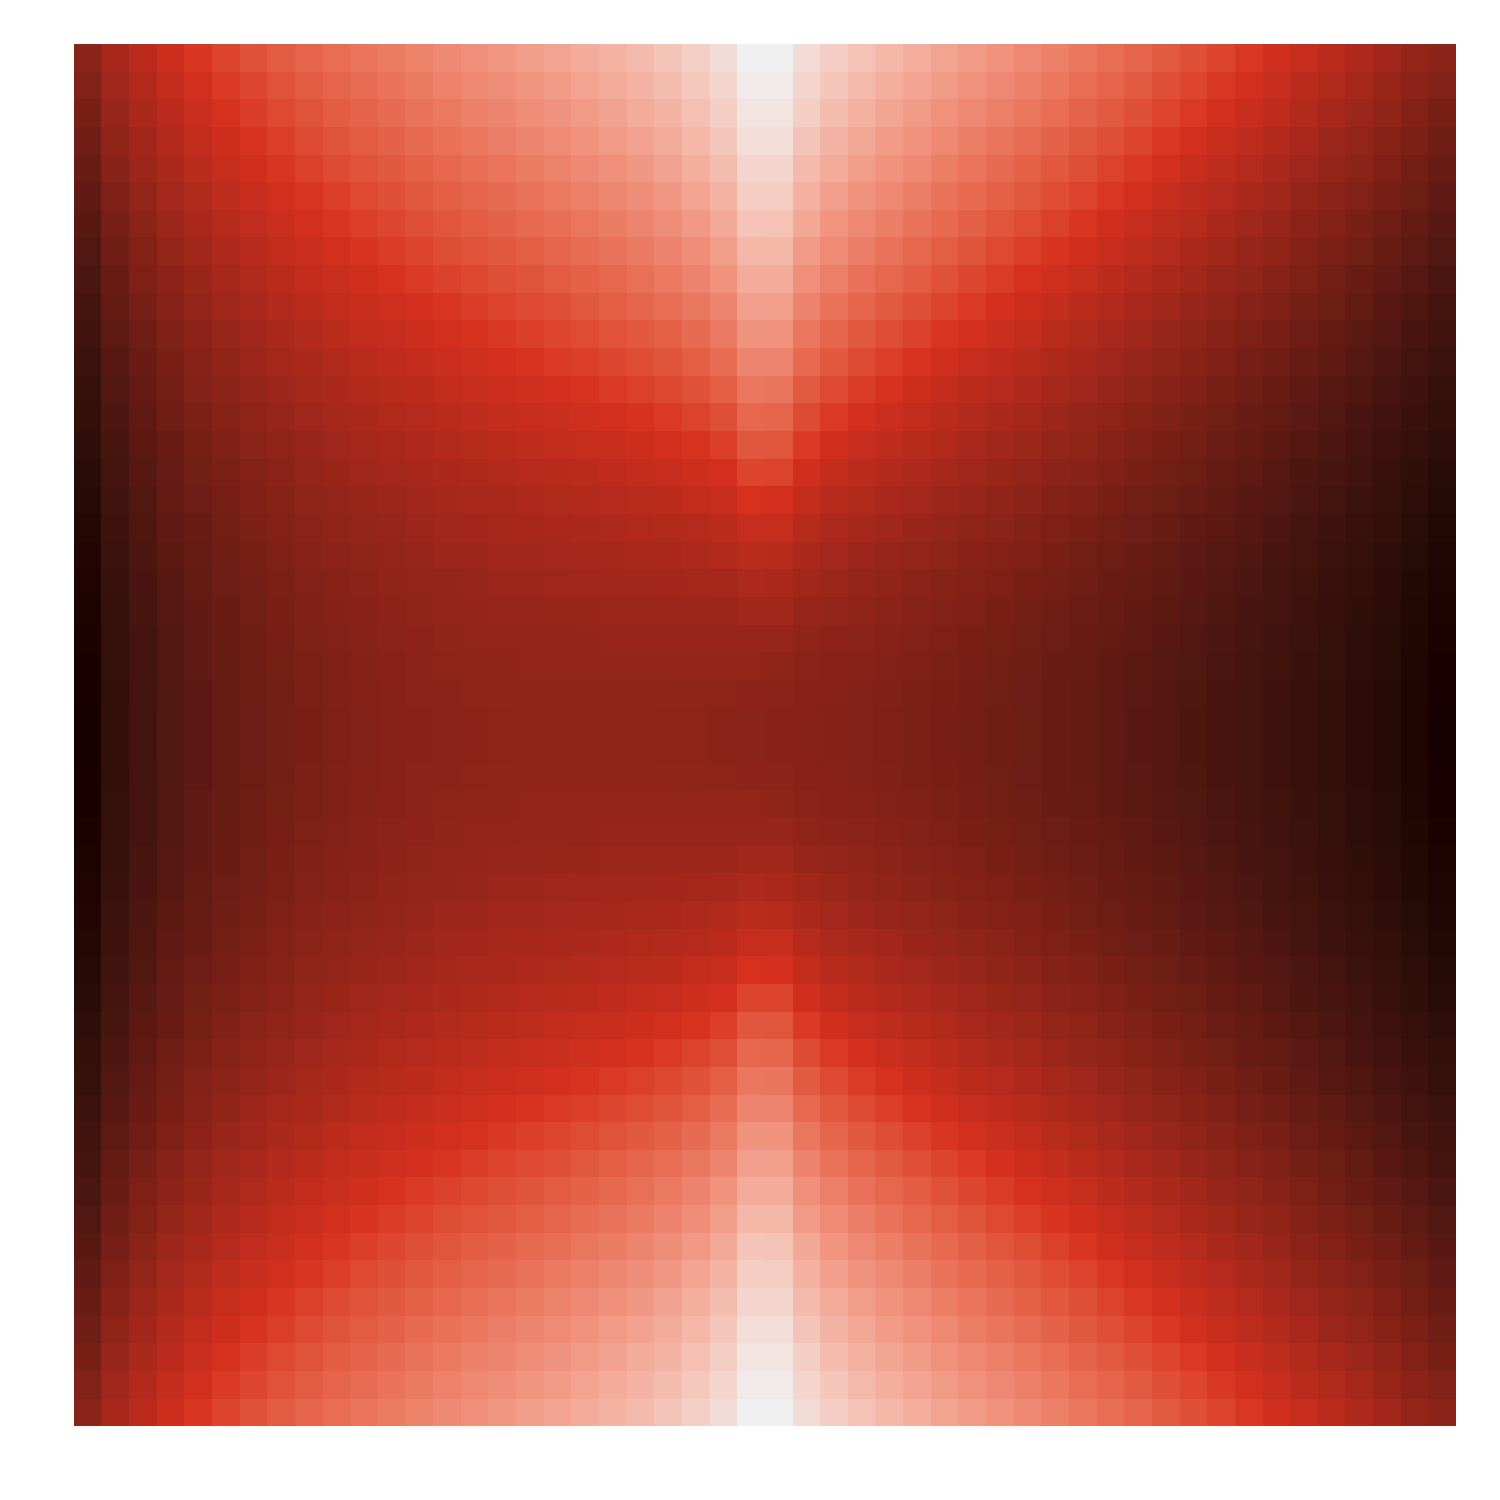
\includegraphics[width=0.32\textwidth]{simulation/documentation/figures/p_smooth6}
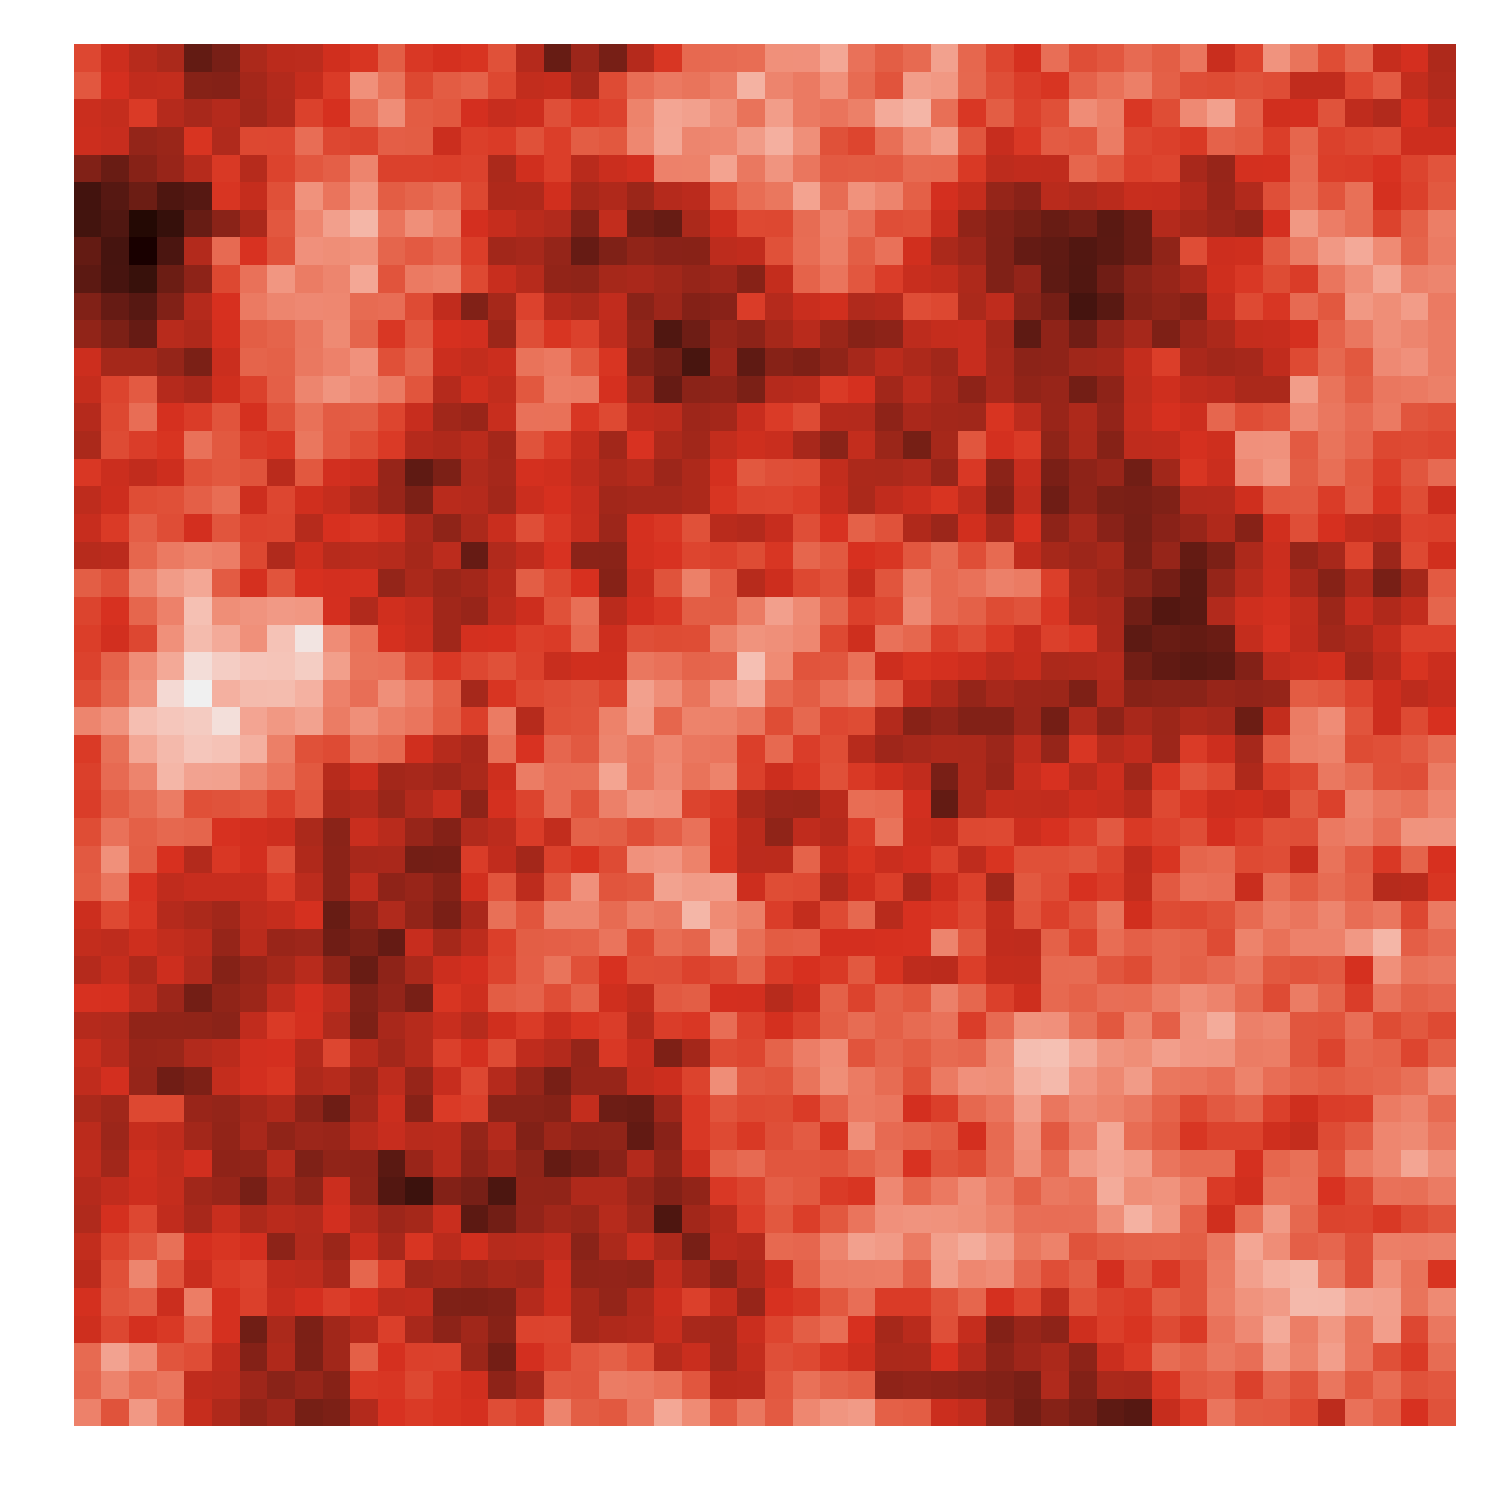
\includegraphics[width=0.32\textwidth]{simulation/documentation/figures/p_realistic4}
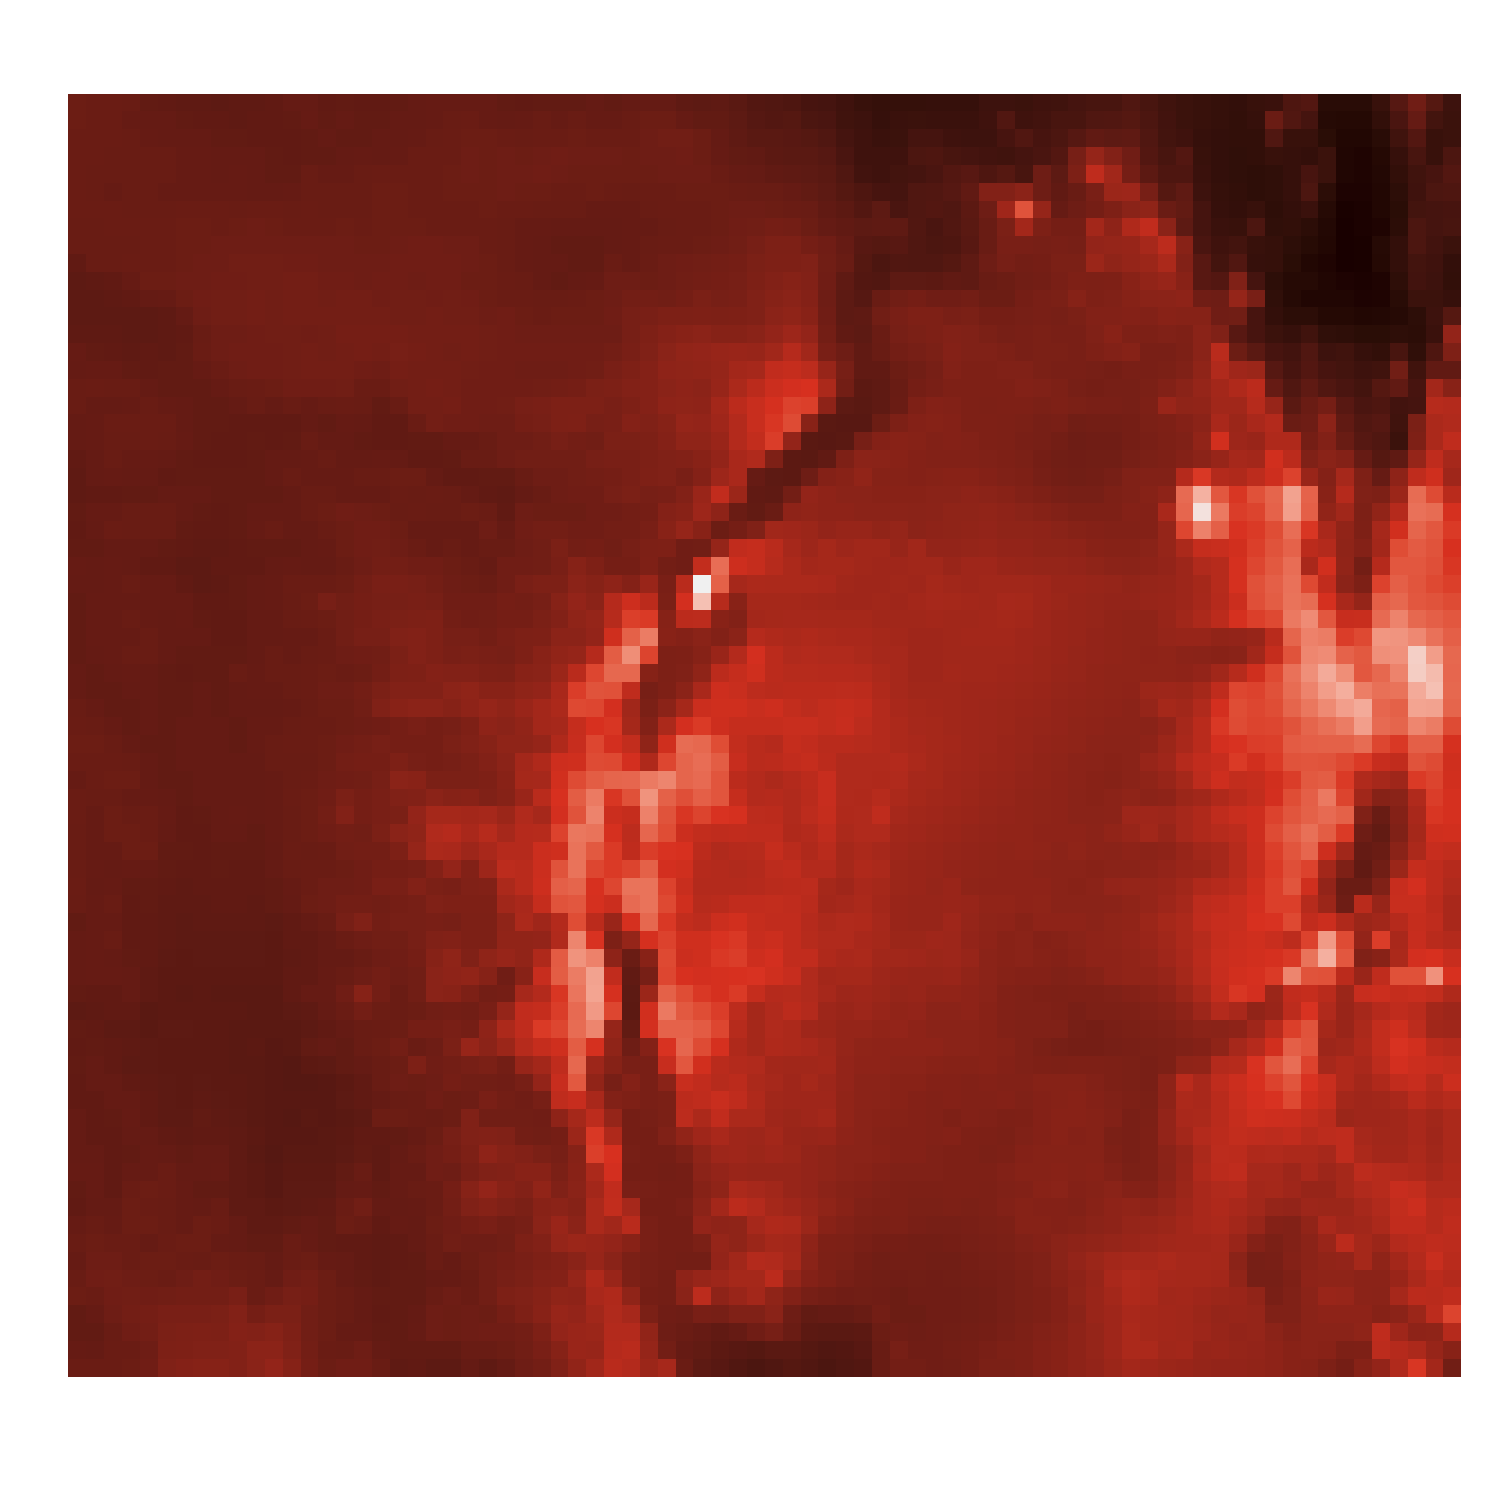
\includegraphics[width=0.35\textwidth]{simulation/documentation/figures/p_real1}
\caption{Illustration of smooth, random and real landscapes as testbeds for simulating spatial autocorrelation. Simulated landscapes are 50 $\times$ 50 pixels, while the real landscape is 72 $\times$ 72 pixels.}
\label{fig:landscapes}
\end{figure}

On these landscapes we simulated different causes of spatial autocorrelation:
\begin{enumerate}
\item[0.] no spatial autocorrelation (as reference);
\item spatial autocorrelation in the error term, i.e. additive at the link scale; this SA should not cause bias of parameter estimates;
\item omitted predictor, which is in itself spatially autocorrelated and hence leaves a SA-signature on the model residuals if not accounted for;
\item wrong functional form: mis-specifying the model by representing a polynomial term only by a linear effect;
\item mass-effect, i.e. spill-over from sites with higher $Y$-values to those around it (representing dispersal).
\end{enumerate}

Finally, all these sets of predictors were used to simulate response variables from three different predictions: Gaussian, Bernoulli and a zero-inflated Poisson. Code for generating all data sets is available in the appendix.

\section{Results}

\section{Discussion}

\noindent Things to comment on:
\begin{itemize}
\item lattice data required (or any spatial positioning of points)?
\item can it be combined with any kind of approach (e.g. with ANN or BRT)?
\item temporal extension possible (e.g. repeated measurements)?
\item mixed-effect model extension possible?
\item data set size (number of cases that can be analysed)
\item time it takes to run a benchmark analysis
\item first shot or best practice method?
\end{itemize}


\noindent R packages doing some kind of spatial regression:
\begin{itemize}
\item \textbf{CARBayes}: ``Spatial Areal Unit Modelling; Implements Bayesian hierarchical spatial areal unit models. In such models the spatial autocorrelation is modelled by a set of random effects, which are assigned a conditional autoregressive (CAR) prior distribution. Examples of the models included are the BYM model as well as a recently developed localised spatial smoothing model.''
\item \textbf{gee}/\textbf{geepack}/\textbf{geesmv}: Generalized Estimation Equation solver.
\item \textbf{geoR}/\textbf{geoRglm}: ``inference in generalised linear spatial models. The posterior and predictive inference is based on Markov chain Monte Carlo methods''
\item \textbf{georob}: ``[F]unctions for fitting linear models with spatially correlated errors by robust and Gaussian Restricted Maximum Likelihood and for computing robust and customary point and block kriging predictions, along with utility functions for cross-validation and for unbiased back-transformation of kriging predictions of log-transformed data.''
\item \textbf{glmmBUGS}: ``Generalised Linear Mixed Models and Spatial Models with WinBUGS, BRugs, or OpenBUGS; write bugs model files for hierarchical and spatial models, arranges unbalanced data in ragged arrays, and creates starting values''
\item \textbf{GWmodel}: Geographically-Weighted Models [see also gwrr, spgwr]
\item \textbf{gwrr}: ``Fits geographically weighted regression (GWR) models and has tools to diagnose and remediate collinearity in the GWR models. Also fits geographically weighted ridge regression (GWRR) and geographically weighted lasso (GWL) models.'' [see also GWmodel, spgwr]
\item \textbf{hglm}
\item \textbf{hGLMMM} (archived)
\item \textbf{hSDM}: e.g. `Binomial logistic regression model with CAR process' for \texttt{hSDM.binomial.iCAR}, or even `to model species distribution including different processes in a hierarchical Bayesian framework: a Poisson suitability process (refering to environmental suitability explaining abundance) which takes into account the spatial dependence of the observations, and a Binomial observability process (refering to various ecological and methodological issues explaining the species detection)' when using \texttt{hSDM.Nmixture.iCAR}
\item \textbf{McSpatial}: ``Nonparametric spatial data analysis. Locally weighted regression, semiparametric and conditionally parametric regression, fourier and cubic spline functions, GMM and linearized spatial logit and probit, k-density functions and counterfactuals, nonparametric quantile regression and conditional density functions, Machado-Mata decomposition for quantile regressions, spatial AR model, repeat sales models, conditionally parametric logit and probit''
\item \textbf{mgcv}: trend-surface regression (with `\texttt{+s(x,y)}', which is similar to SEVM, really); GLS-like with correlation structures from \textbf{nlme}
\item \textbf{ngspatial}: ``[T]ools for analyzing spatial data, especially non-Gaussian areal data. The current version supports the sparse spatial generalized linear mixed model [...] and the centered autologistic model''
\item \textbf{nlme}: fits GLS and mixed effect models, including a spatially structure variance-covariance matrix
\item \textbf{PReMiuM}: ``Bayesian clustering using a Dirichlet process mixture model. This model is an alternative to regression models, non-parametrically linking a response vector to covariate data through cluster membership. The package allows Bernoulli, Binomial, Poisson, Normal, survival and categorical response, as well as Normal and discrete covariates. It also allows for fixed effects in the response model, where a spatial CAR (conditional autoregressive) term can be also included.''
\item \textbf{ramps}: ``Bayesian geostatistical modeling of Gaussian processes using a reparameterized and marginalized posterior sampling (RAMPS) algorithm designed to lower autocorrelation in MCMC samples. Package performance is tuned for large spatial datasets.''
\item \textbf{R-INLA}: ``solves models using Integrated nested Laplace approximation (INLA) which is a new approach to statistical inference for latent Gaussian Markov random field (GMRF) models''
\item \textbf{regress} with \textbf{spatialCovariance}: ``Functions to fit Gaussian linear model by maximising the residual log likelihood where the covariance structure can be written as a linear combination of known matrices. Can be used for multivariate models and random effects models. Easy straight forward manner to specify random effects models, including random interactions''
\item \textbf{spaMM}: ``Implements a collection of functions for inference in mixed models. It was developed in particular for GLMMs with spatial correlations.''
\item \textbf{spatcounts}: ``Fit spatial CAR count regression models using MCMC''
\item \textbf{SpatialFA}: Spatial factor analysis for joint species distribution modelling (unclear whether useful as spatial model)
\item \textbf{spatialprobit}: ``spatialprobit: Spatial Probit Models; Bayesian Estimation of Spatial Probit and Tobit Models''
\item \textbf{spdep}: ``[F]unctions for estimating spatial simultaneous autoregressive (SAR) lag and error models, impact measures for lag models, weighted and unweighted SAR and CAR spatial regression models, semi-parametric and Moran eigenvector spatial filtering, GM SAR error models, and generalized spatial two stage least squares models.''
\item \textbf{spgwr}: Geographically weighted regression [see also GWmodel, gwrr]
\item \textbf{sphet}: ``Generalized Method of Moment estimation of Cliff-Ord-type spatial autoregressive models with and without heteroscedastic innovations''
\item \textbf{stocc}: ``fits spatial occupancy models'', but you can also use it for single-visit analyses (see here for an example: \url{rstudio-pubs-static.s3.amazonaws.com/9687_cc323b60e5d542449563ff1142163f05.html})
\end{itemize}
%
Other software: \textbf{SAM}, Geo/Win/Open\textbf{BUGS}



\section{Benchmark data sets}
Potential \textbf{causes} of spatial autocorrelation to be simulated:
\begin{enumerate}
\item[0.] no SA as reference (would these methods over-compensate?)
\item unbiased spatial autocorrelation error term (as in snouters);
\item omitted predictor (this can represent an unmeasured environmental predictor, or a sampling bias, or a biotic interaction affecting occurrence); 
\item wrong functional form (i.e. the model must miss a quadratic term or interaction; \emph{not} something we can provide in the data, except by simulating data that have non-linear functions and interactions);
\item mass-effect spatial autocorrelation (i.e. dispersal from occupied sites onto those around (only \emph{increasing} $P(X=1)$, not decreasing it; this would mean that suitable sites spill over into unsuitable).
\end{enumerate}
%
\textbf{Data simulation}:\\
(The idea is to make an R-package from the data simulation step and have the 315 data sets to be generated as argument. So if somebody writes \verb|makeData("311")|, sHe will get exactly the data set we used, along with a description of all parameters and settings!)\\
(I would start on the minimal set, possibly with made-up environmental data instead, but have the whole thing in mind!)
\begin{enumerate}
\item kind of environmental data: (a) linear and non-linear gradients without noise; (b) Gaussian field-generated ``realistic landscapes''; (c) real data (e.g. bioclim, 2000 x 2000 km at 20 km resolution) for central Africa\footnote{\url{http://www.ncgia.ucsb.edu/conf/SANTA_FE_CD-ROM/sf_papers/hutchinson_michael_africa/africa.html}\\Why Africa? For several reasons: (1) it is near the equator, so we can use the data without reprojection to equal-area; (2) Africa is neglected; (3) it has nice strong climatic gradients; (4) virtually no-one has a preconception of effects there; (5) it is large enough to cut out a 4e6 km$^2$ chunk. My idea of coordinates: 5N24E to 7S37E or so.}, with an east-west temp-gradient and a north-south rain-gradient; low to no correlation between predictors! (this is not about collinearity)
\item response complexity: moderate only, incl. X1, X2, X2\^{}2, X1:X2, X3, X3\^{}2 as actual predictors and X4-X7 as nuisances;
\item response variable: Gaussian, Bernoulli, zero-inflated Poisson (i.e. mixing the Bernoulli and a Poisson); relatively low noise on Gaussian;
\item size: generate landscapes of 100$\times$100 cells, then down-sample to differently sized data sets: 100, 200, 500, 1000, 2000, 5000, 10000; additionally 1E6 data to check `big data' suitability; all sampled regularly from the full-resolution 100$\times$100 grid.
\item validation: provide a 10-fold block-cross-validation fold ID for each data set
\end{enumerate}
%
\textbf{Data analysis}:
\begin{itemize}
\item run all analysis with default settings, then contact authors to improve; don't tell them the real parameters, nor which predictors are relevant, but give them the correct functional form (i.e. quadratic terms and interactions, except for the purposefully wrong data sets); \textbf{no model selection!} (because that will lead to biased estimates and hence makes the incomparable)
\item extract: parameter estimates for each CV; RMSE on each 10-fold block cross-validation; effect plots for one or two selected predictors for each CV; model residuals on the link scale for each CV
\item provide data sets of different size and record computing times: what is feasible with which method?
\end{itemize}
%
Full \textbf{number of data sets}: 5 causes * 3 landscapes * 3 distributions * 7 sizes = 315 data sets; \\
Minimal set: 2 causes (1 and 2) * 1 landscape (real) * 2 distributions (Gaussian and Bernoulli) * 1 size (1000) = 4 data sets;




\bibliographystyle{apalike2} %apalike2 hat ein "&" statt eines "and" zwischen den Authoren!
\bibliography{../../../LiteratureOrganisation/CFD_library}
\end{document}  